
\section{Jets}
 {\color{blue}        (10 pages)}
 
 
\begin{figure}[t]
 \centering
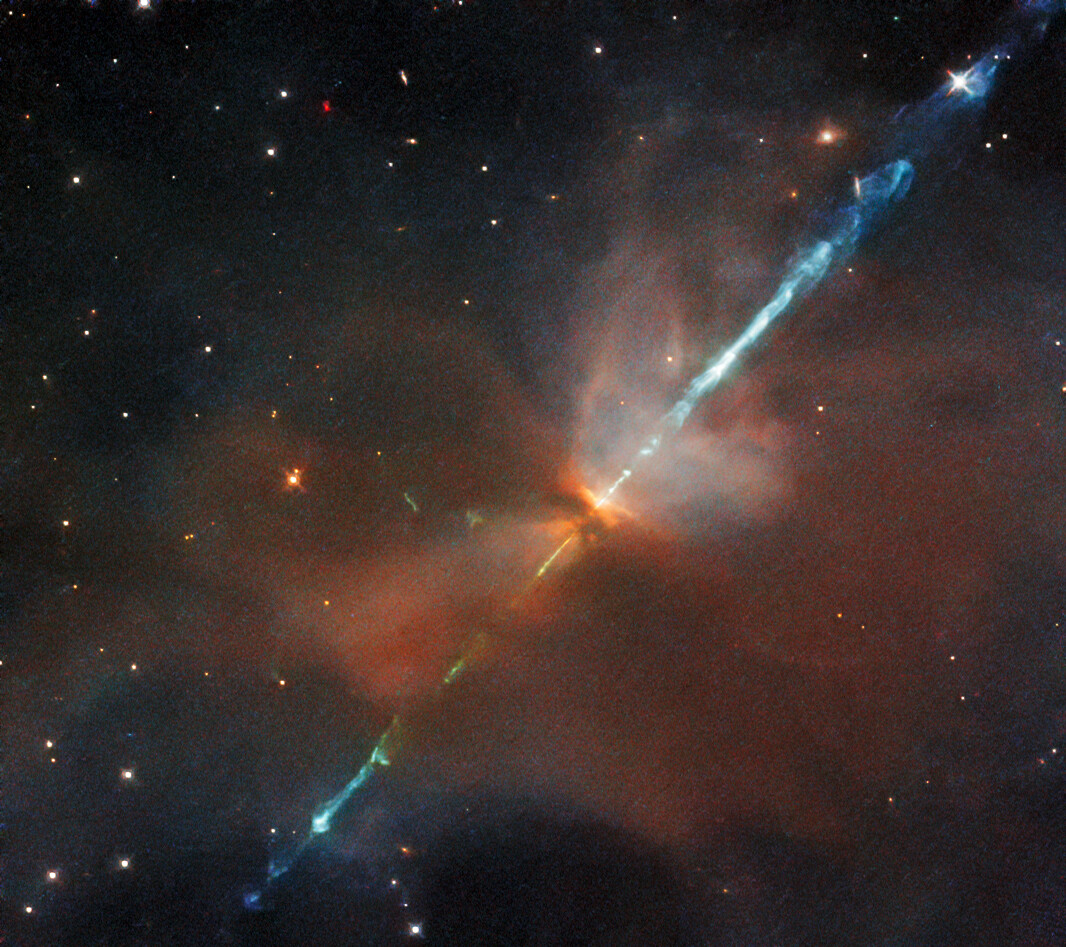
\includegraphics[width=6cm]{figs/HH111_-_HST_-_Potw2135a.jpg}
\caption{HST composite image of HH~111. Image credit: ESA/Hubble & NASA, B. Nisini. \label{fig:HH111} }
\end{figure}
 
 
% https://en.wikipedia.org/wiki/File:HH111_-_HST_-_Potw2135a.jpg 
 
A variety of mass ejection phenomena occur during the first stages of star evolution which are intimately related to the accretion process described in the previous section. In general, plasma is ejected from a young stellar system, which then propagates in the ambient medium with supersonic velocities. Outflows in pre-main sequence stars (PMS) are detected in a wide range of wavelengths and show very different morphologies, from jets to less-collimated, wide-angle outflows. In this section, we focus on protostellar jets which are well collimated beams (opening angles of a few degree) 

Most jet observations are compatible with MHD winds launched from the inner regions of protoplanetary disks \citep{Frank_2014}. However, there are other possible launch regions. First, stellar winds launched from the hot stellar corona much like the solar wind \citep{Matt_2005}. In analogy with the solar wind, such stellar winds are very hot ($\gtrsim10^6$\,K) and may cool via X-ray emission. Second, magnetospheric ejections launched from the region between the star and the inner edge of the disk \citep{Zanni_2013}. Third, X-winds are launched from a narrow region close to the inner edge of the disk \citep{Shu_1994}. Even more mechanisms to launch outflows may exist  in the young, class~0 objects, but they produce slower outflow velocities and are therefore related to the observed X-ray emission and ignored here.
 
{\color{red} TBD: Magnetic towers \citep{Huarte_2012}? }

Observationally,  protostellar outflows  were ``discovered''\footnote{The nebulosity around T~Tau was first described in the 19th century  by \citet{Burnham_1890, Burnham_1894}.} by \citet{Herbig_1950,Herbig_1951} and \citet{Haro_1952,Haro_1953}. These authors studied the optical, nebular emission, mostly from forbidden emission lines (FELs), which is typically concentrated in individual, relatively distinct emission regions along the jet path and these so-called knots or chains of knots are called Herbig-Haro (HH) objects (see Fig.~\ref{fig:HH111} for a beautiful example). Protostellar jets are bright in FELs, because shocks within the outflow heat the outflowing plasma to temperatures of roughly $10^4\,$K \citep{}. According to Eq.~\ref{eqn:Tshock}, such a post shock temperature corresponds to shock velocities of $\sim20-30$\,km\,s$^{-1}$.
%
Because of the low densities ($\lesssim10^4\,$cm$^{-3}$ beyond few tens of au), radiative cooling of the shock heated plasma is dominated by hydrogen (e.g., H$\alpha$) and metalic forbidden emission lines like [O~{\sc i}], [S~{\sc ii}], and [Fe~{\sc ii}]. These lines (or line ratios) allow one to estimate the physical properties of the emitting plasma \citep[temperature, density, ionization degree, e.g., ][]{Bacciotti_1999}.

Since their discovery, protostellar jets were studied in a variety of wavelengths, from radio \citep{} to (near-) IR \citep{}. However, there were simply no indications for plasma temperatures well in excess of several tens of thousands of K; emission from [O~{\sc iii}] were considered ``high-ioniziation'' in the protostellar jet context. Hence, the detection of protostellar jets in X-rays came to a surprise.

\subsection{X-rays from protostellar jets}


% 
% \begin{figure}[t]
% \centering
% 
% 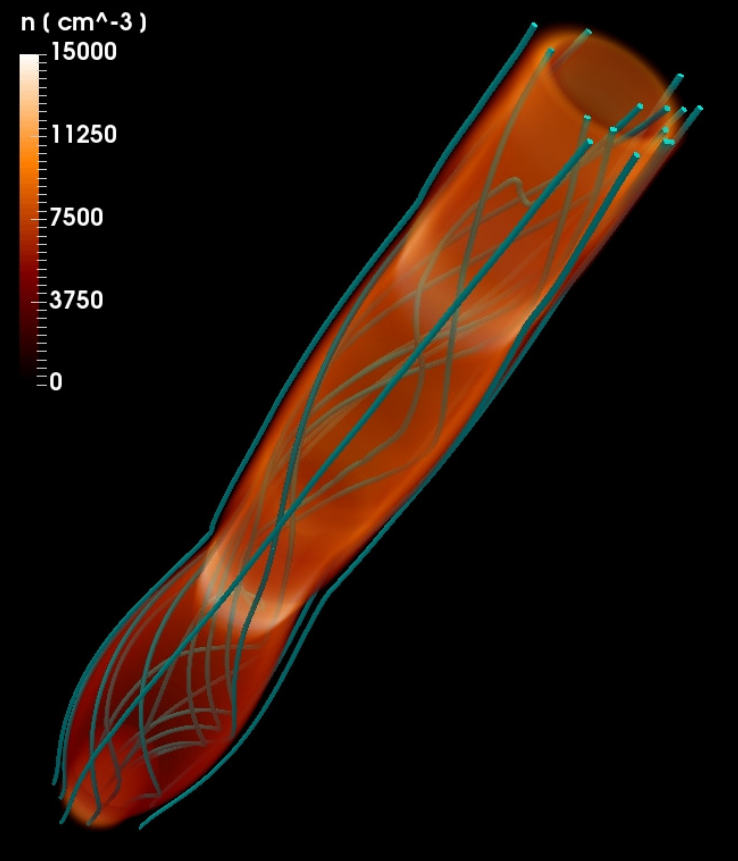
\includegraphics[height=6cm]{figs/diamond}
% % % % 
% %  \vspace*{-0.5cm}
%  %
%  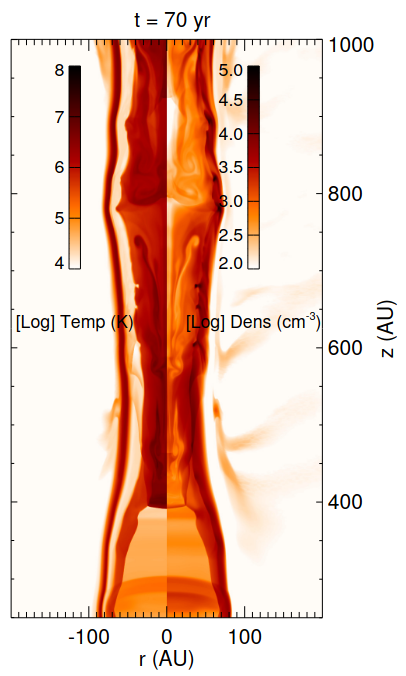
\includegraphics[height=7cm]{figs/diamond_simu}
% 
% \caption{{\bf Left: } Structure of jet and magnetic field close to the base. From \citet{Ustamujic_2016}.
%          {\bf Right: }. From \citet{Ustamujic_2018}. \label{fig:jet_simu}}
% \end{figure}




\begin{figure}[t]
\centering

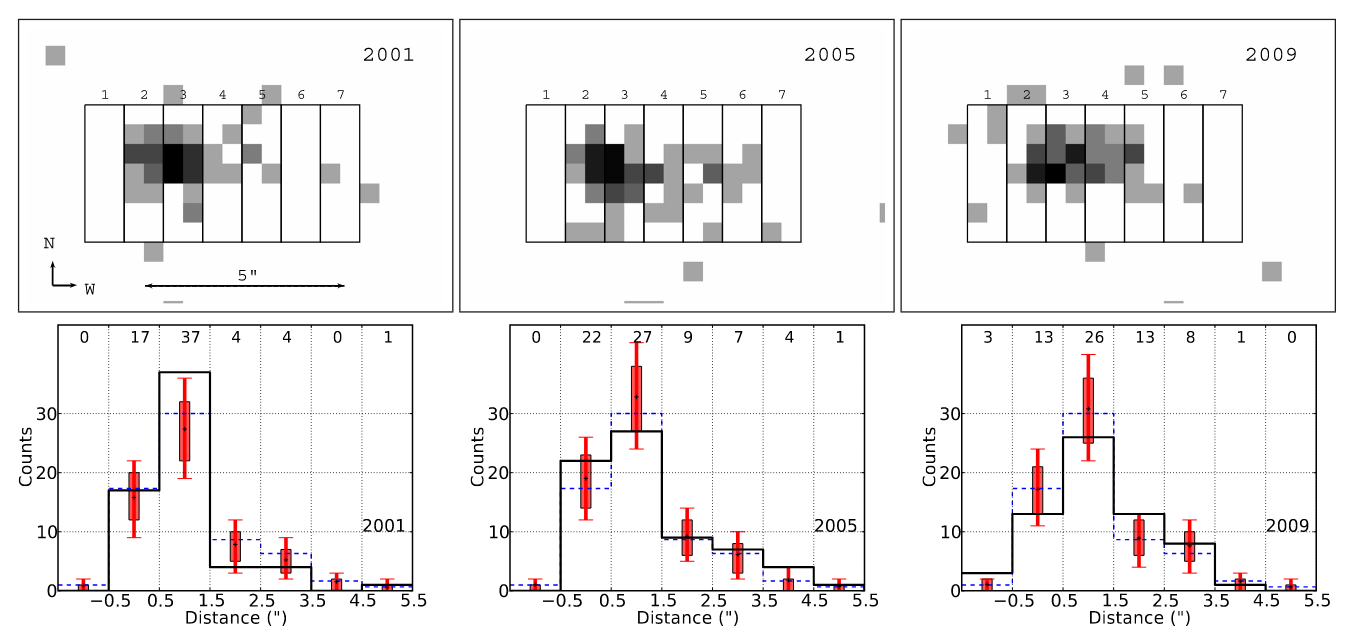
\includegraphics[height=6cm]{figs/hh154}
% % % 
\caption{Evolution of the X-ray emission from HH 154. From \citet{Schneider_2011}. \label{fig:hh154}}
\end{figure}


% \subsection{X-ray jet observations}
The first X-ray detections of protostellar jets were obtained almost simultaneously in 2001 by \citet{Pravdo_2001} using Chandra (HH~2) and \citet{Favata_2002}
using XMM-Newton (HH~154 or L~1551~IRS\,5). Both HH objects are launched from class~I objects. The association of the Chandra detected X-ray emission to HH~2 straight forward, because the X-ray emission  (a) spatially coincides with one of the optically brightest knots within HH~2, (b) appears extended, and (c) the spectrum is soft ($T\sim1.2\times10^6\,$K) unlike typical coronae of young stars. In contrast, the association of the X-rays from the L\,1551~IRS\,5 complex to HH~154 strongly builds on the severe extinction towards the protostellar sources while the jet suffers much less extinction \citep[$A_V(jet)\sim10\,$mag vs $A_V(protostars)\gtrsim150$\,mag, e.g.,][]{White_2000,Fridlund_2005}. This high $A_V$ towards the stellar sources led \citet{Favata_2002} to ascribe the X-rays to HH~154 despite the proximity of the X-ray emission with the stellar position and the comparably high mean X-ray energies ($\sim1\,$keV), simply because any reasonable X-ray emission from the stellar system would not make it directly to the observer. Later, \citet{Bally_2003} located the X-rays from HH~154 to the base of the outflow using new Chandra data but also find a higher temperature for the emitting plasma and, thus, reconsider the origin of the X-rays discussing reflection of stellar X-rays from one (or a combination) of the protostars by some medium close to the stars and a variety of shocks, e.g., within the outflow, against one disk, or between the stellar winds of the individual protostars of the system. These authors already note that the location of the X-rays may be in a region where the outflow is collimated to the narrow jet observed further away from the sources, which turned out to be, at least obserationally, a relatively common feature and the X-ray emission of protostellar jets can be broadly divided into emission from the jet base and from working surfaces at large distances to the driving sources.

X-ray emission close to the base of the jet, and far away (HH objects) also due to interaction with dense CSM or molecular clouds.
 

 
\subsubsection{X-rays from the jet base}



 
\begin{figure}
    \centering
    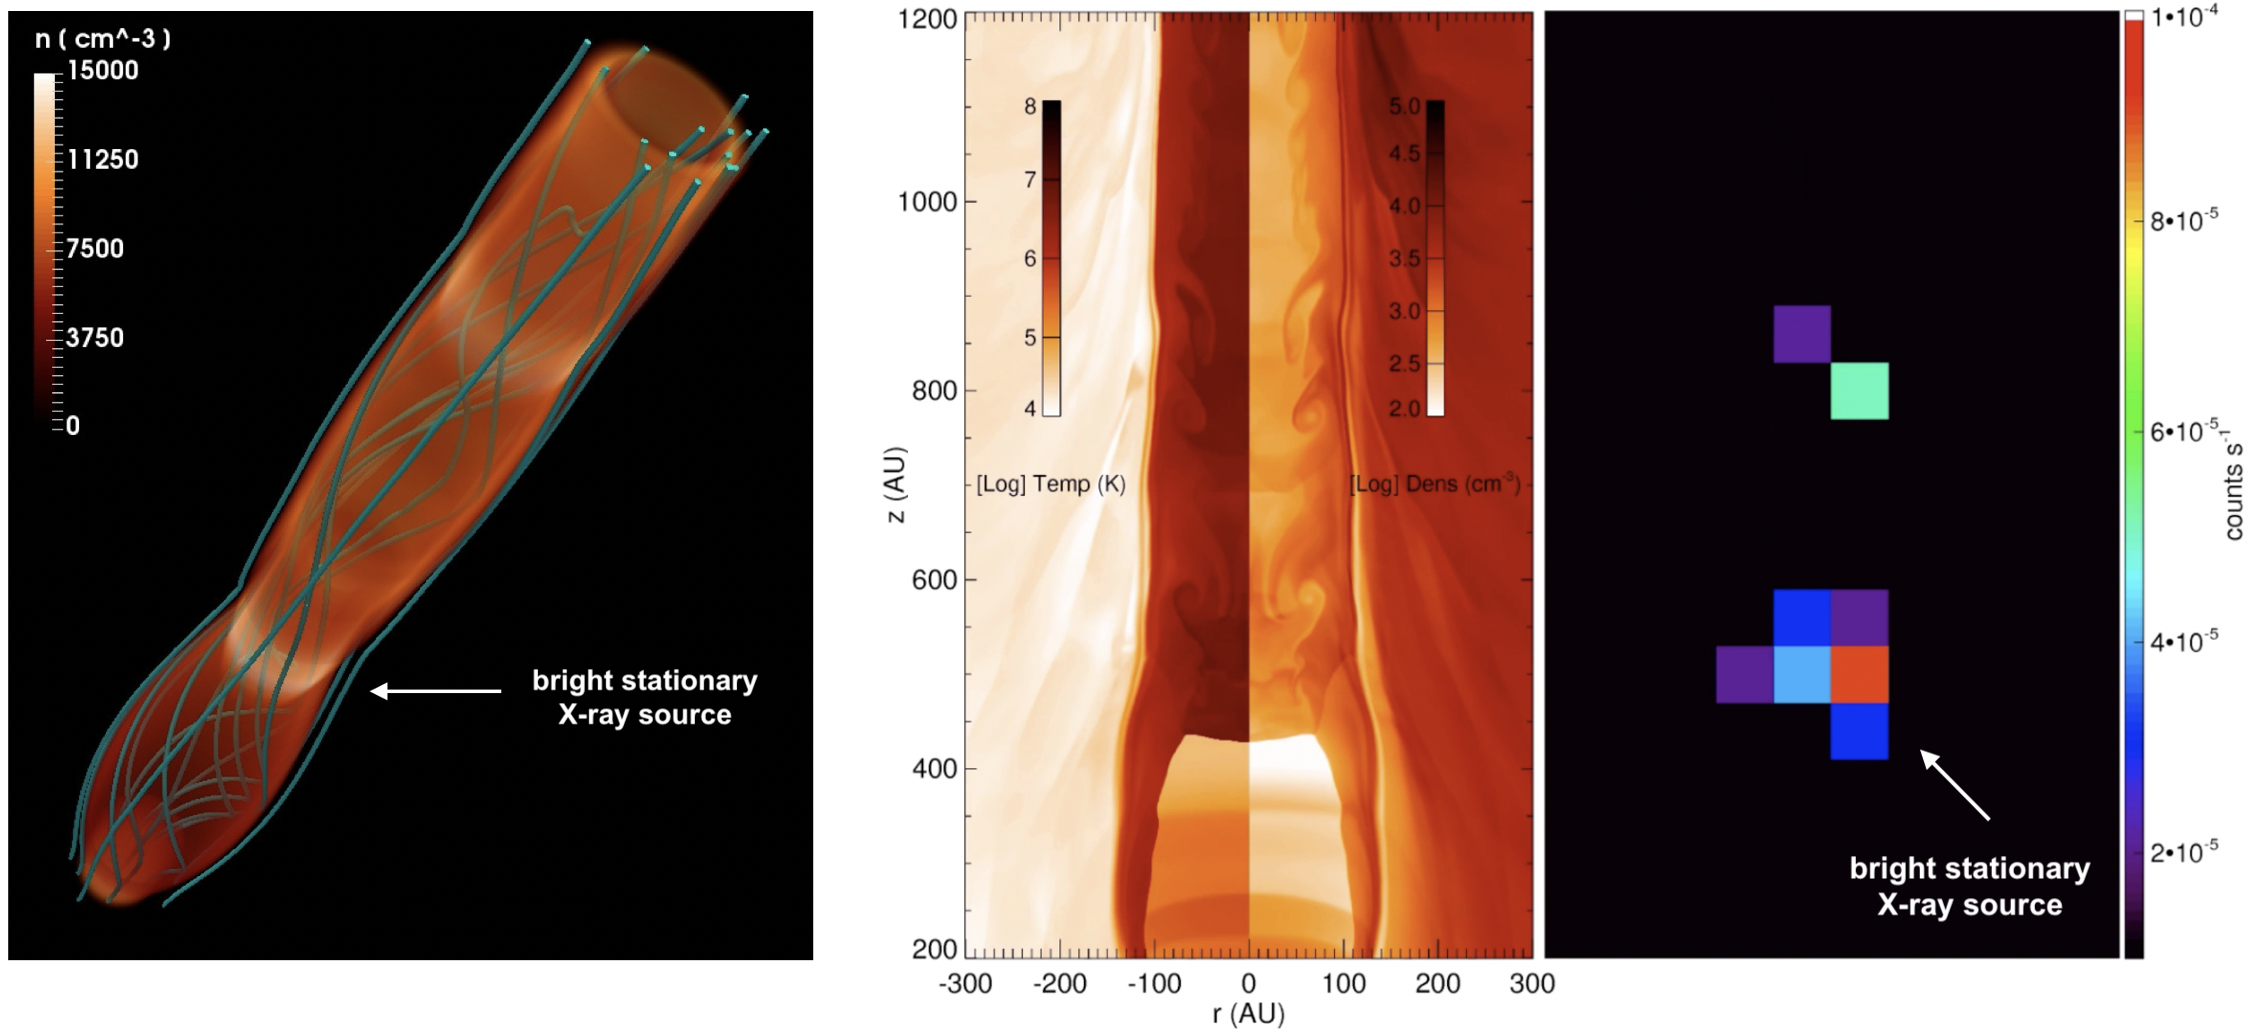
\includegraphics[width=12cm]{figs/ustamujic.png}
    \caption{A combination of Figs. from Ustamujic et al. 2016,2018,2019. I'd rather prefer this one in order to include the X-ray emission synthesized from the model (which is in agreement with the observations).}
    \label{fig:ustamujic}
\end{figure}



\begin{figure}[t]
% \centering

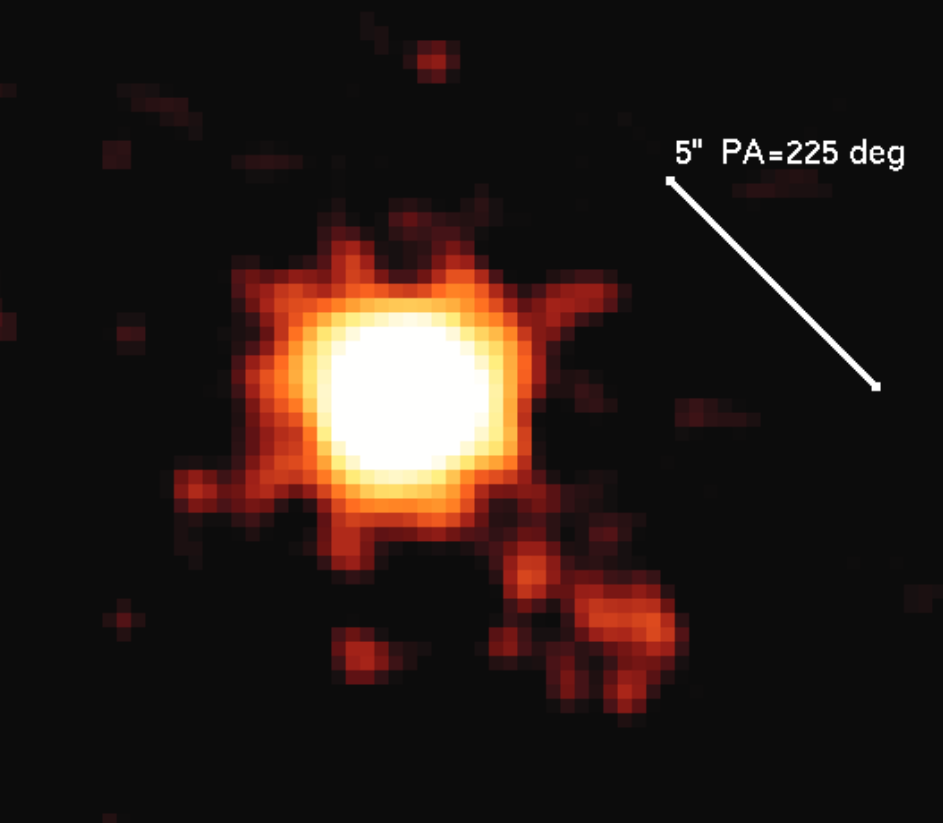
\includegraphics[width=6cm]{figs/dg_tau_X}
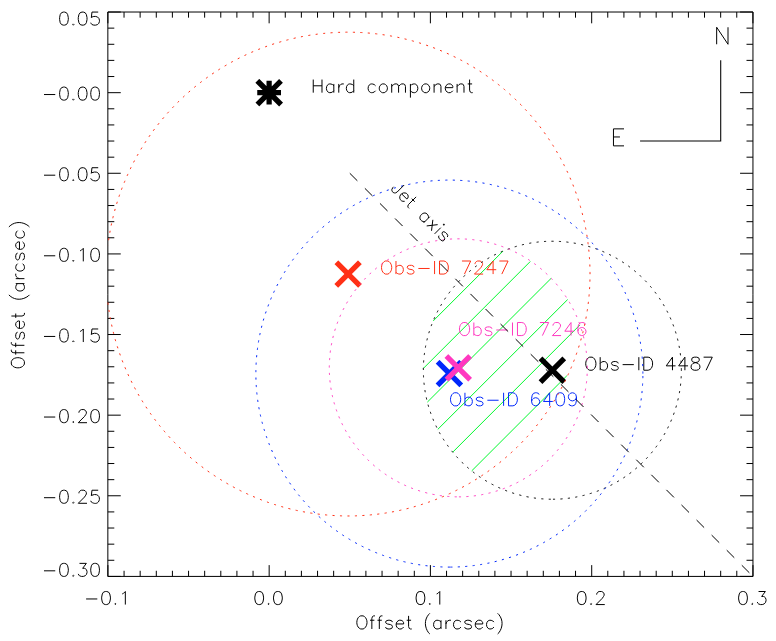
\includegraphics[width=6cm]{figs/dg_tau_offsets}

\caption{{\bf Left: } Chandra X-ray image of the DG~Tau system. From \citet{2011ASPC..448..617G}.
         {\bf Right: } Relative spatial offsets between the hard (coronal) and soft (jet) emission. From \citet{Schneider_2008}. \label{fig:dg_tau_X}}
\end{figure}


\subsubsection{X-rays from jet knots}

{\color{blue}(jet origin, collimation, jet velocities) [Christian, Sabina]}


Sketch (suggestion?) should we make a new sketch? Is Fig.~\ref{fig:jet_simu} left sufficient?
I think that it's sufficient. If we have enough space I would separate the panels in two figures: left panel to talk about the physics and the right one for the X-ray emission from jets.

Wind, outflows and jets: Bally 2016 (main components of outflows); Matt \& Pudritz 2005 (accretion powered winds), Zanni \& Ferreira 2013 (magnetospheric ejections)

Jet origin, ejection and collimation here.
MHD model magnetospheric ejections Zanni \& Ferreira 2013

\begin{figure}
    \centering
    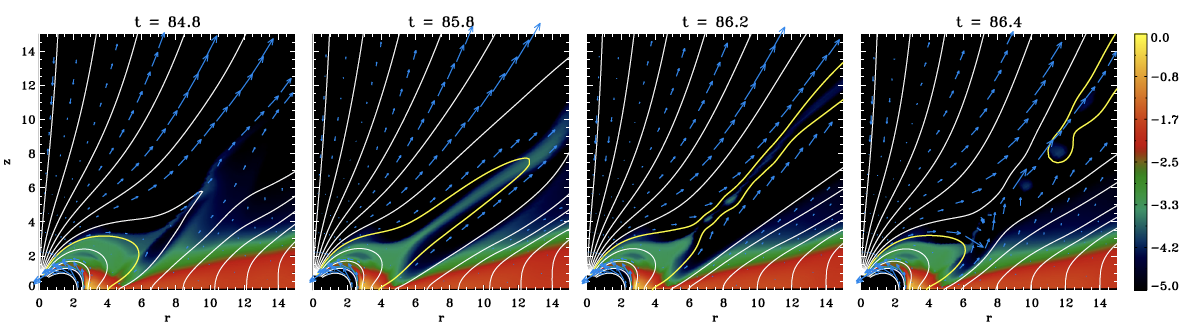
\includegraphics[width=12cm]{figs/Zanni2013.png}
    \caption{Temporal evolution of the periodic inflation/reconnection process which characterizes the dynamics of the magnetospheric ejections. Need to ask for permission.}
    \label{fig:zanni2013}
\end{figure}

{\color{blue}Christian

Favata HH 154, Guedel DG Tau, Schneider HH 154

Laboratory experiments  e.g. Revet et al. 2017
}

X-ray discovered jets: HH 2 \citep{Pravdo_2001,Schneider_2012}, HH 154 \citep{Favata_2002,Bally_2003,Favata_2006,Schneider_2011}, HH 168 \citep{Pravdo_2005,Schneider_2009}, DG Tau \citep{Guedel_2005,Guedel_2008,Schneider_2008}, Z CMa \citep{Stelzer_2009}, RY Lup \citep{Skinner_2011}, HD~163296 \citep{Swartz_2005,Guenther_2013}, TAX \citep{Guedel_2007}, HH~80/81 \citep{Pravdo_2004}, HH~210 \citep{Grosso_2006}, HH~248 \citep{Lopez_2015}.

\subsection{Models of jets}

A paragraph about models to study the launching site.

Different scales

\subsubsection{Modelling of X-ray emitting jets}
\citet{Raga_2002}

HD models (Bonito), MHD (Ustamujic) and comparison with observations

X-ray emitting close to the base
Far away

\subsubsection{Mass loss rate}

\subsection{Plasma cooling \label{sect:cooling}}
Three processes contribute to the cooling of a plasma: Radiative cooling, cooling by expansion and thermal conduction.
The pressure work done by the plasma is $\delta W = p dV$ and the radiative losses are
\begin{equation}
\delta Q_{rad} = -n_e^2 V(t) \Lambda(T) dt\,,
\end{equation}
where $n_e$ is the electron density, $V$ the volume and $\Lambda(T)$ is the cooling function.
The conductive heat flux is given by
\begin{equation}
q_{cond} = -\kappa(T)\bigtriangledown T\,, \label{eq:cond}
\end{equation}
where the thermal conductivity according to Spitzer is
\begin{equation}
\kappa(T) = \kappa_0 \frac{T^{5/2}}{\ln \Lambda}\;\mbox{erg}\,\mbox{s}^{-1}\,\mbox{K}^{-1}\,\mbox{cm}
\end{equation}
with $\kappa_0=1.8\times10^{-5}$ and the Coulomb logarithm $\ln \Lambda$, which describes the collision properties of the plasma and is of order 10.
When the mean free path length for energy exchange is of the same order as the thermal scale height, the conduction should be approximated by the saturated flux
\begin{equation}
q_{sat} = 5 \phi \rho c_s^3\,,
\end{equation}
with $\phi\approx0.3$ \citep[e.g.][$\rho$ is the mass density and $c_s$ is the local sound speed]{Borkowski_1989}. For an estimate of the importance of the saturated flux, we assumed a linear temperature decrease. Under these circumstances the Spitzer value  exceeds the saturated flux on spatial scales of about 10\,AU for the cooling from $T_1=10^6$~K to $T_0=10^4$~K, i.e., the saturated flux should be used for these steep gradients ($n\approx10^3$).



Thermodynamics states that the energy change of a plasma cell is described by
\begin{equation}
dU + \delta W = \delta Q = \delta Q_{rad} + q_{cond}\cdot A\;dt\; \label{eq:cooling1}
\end{equation}
with the internal energy $U=\alpha N kT$ ($\alpha=3/2$ for a fully ionized plasma), the particle number $N$, the Boltzmann constant $k$, the temperature $T$  and $A$ is the surface area through which heat conduction proceeds.
We use $p=2n_ekT$ in the expression for the pressure work and follow \citet{Guedel_2008} by writing  eq.~\ref{eq:cooling1} as
\begin{equation}
\alpha \frac{dT}{T(t)} + \frac{dV}{V} = - \left( \frac{n_e \Lambda(T)}{2 k T(t)}+ \frac{\kappa_0}{2n_eVkT}\cdot A\frac{T^{5/2}}{\ln \Lambda} \nabla T \right) dt \,,\label{eq:cool}
\end{equation}
where we used $N_e=n_e\cdot V$ and note that this expression holds only in the presence of sufficiently small temperature gradients.


In order to estimate the relative importance of the three cooling terms, additional information is needed, in particular, the opening angle of the X-ray emitting jet, its density structure, the temperature gradient, the surface for the heat conduction, which would include the magnetic topology and the properties of the environment, e.g., its ionization. These quantities are not available for the X-ray emitting part of the jet. We therefore decided to give some order of magnitude estimates for the cooling times of the individual processes ignoring contributions of the other ones. As we will see, there are distinct regions in the parameter space where each process seems ApJ...576L.149Rto dominate, so we regard this approach reasonable.

Figure~\ref{fig:cooling} shows the cooling curves for the different processes assuming different parameters for the jet. For radiative and conductive cooling, the mapping of time to distance in this figure depends on the actual, deprojected space velocity of the plasma. 
A rough estimate is 0.3\arcsec{}~yr$^{-1}$, which implies that today's inner X-ray emission will reach the position of today's outer emission in 15 years.
Adiabatic cooling, on the other hand, does not depend of the outflow velocity but only on the initial cross-section of the plasma and on the opening angle.


\begin{figure}
  \centering
   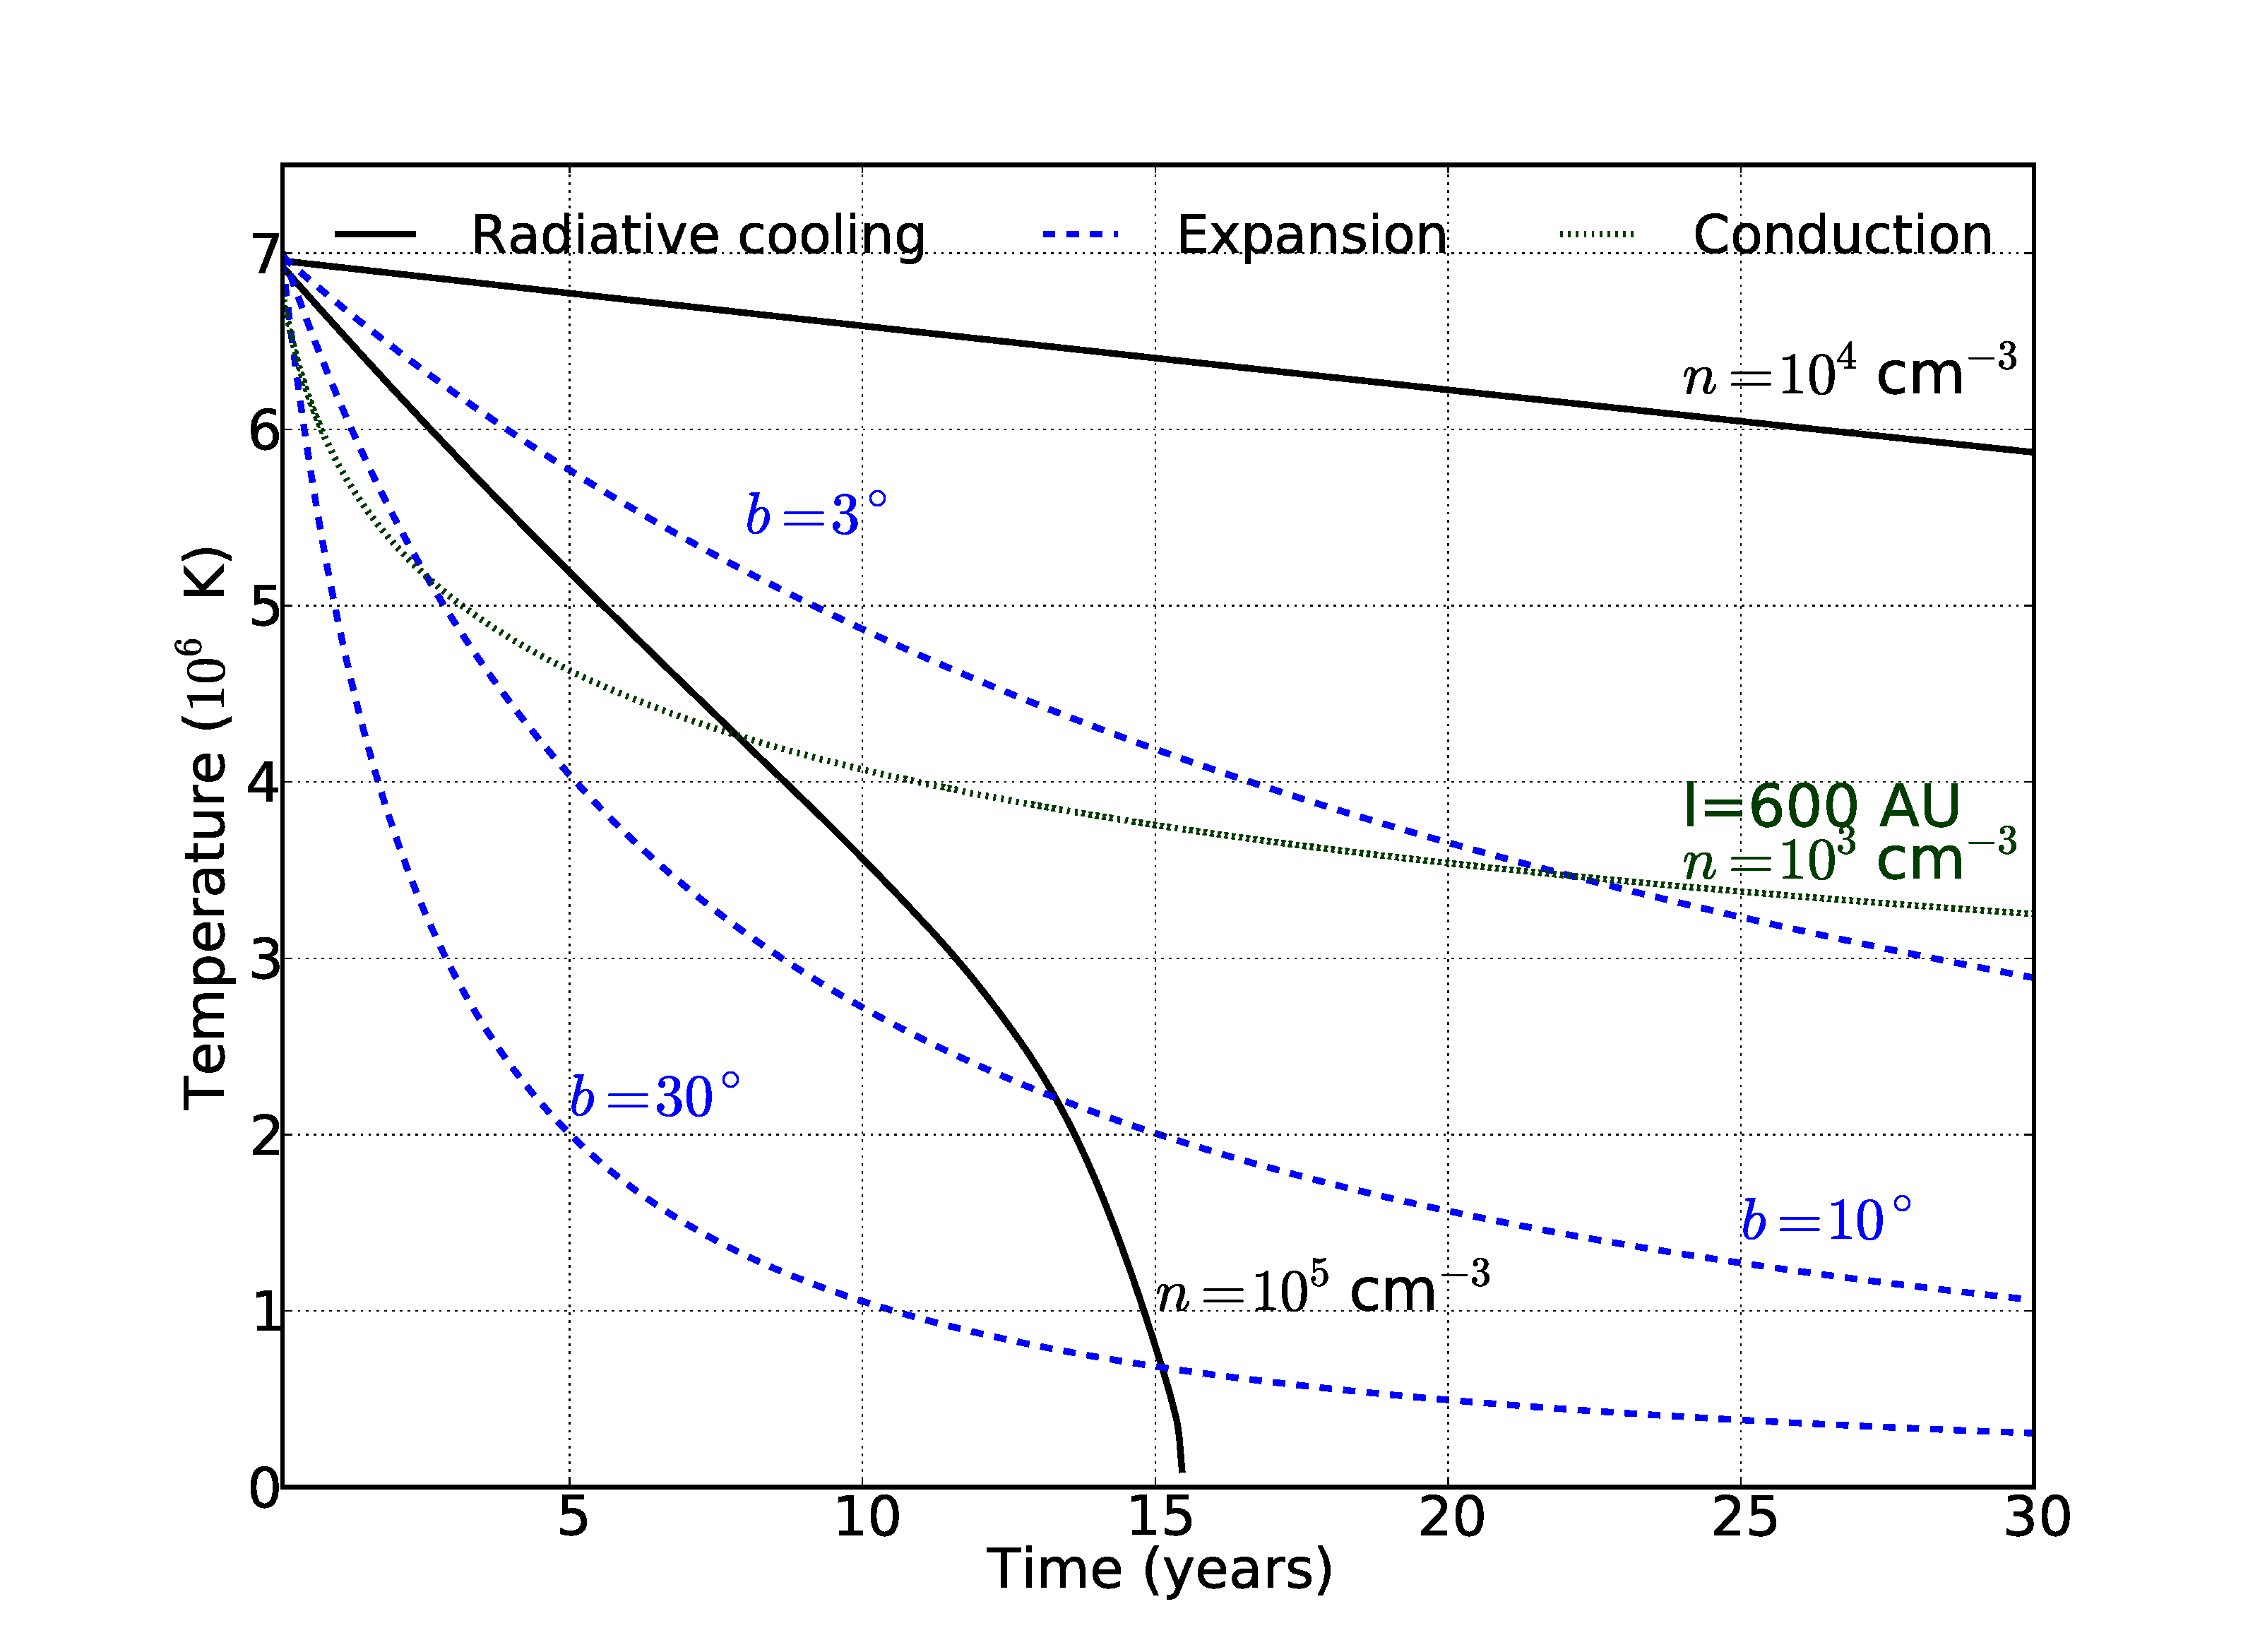
\includegraphics[width=0.49\textwidth]{figures/cool.eps}
   \caption{Cooling curves for the different cooling processes. Parameters of the models are labeled (density: $n$, opening angle: $b$, cooling length: $l$). \label{fig:cooling}}
\end{figure}


\subsubsection{Adiabatic cooling\label{sect:aCooling}}
Protostellar jets usually show an approximately conical structure at some distance from the driving sources so that the flow expands mainly perpendicular to the jet axis.
In the limit of adiabatic cooling
\begin{equation}
T\,V^{\gamma-1} = \mbox{const}
\end{equation}
holds. Since we do not observe local temperatures, we have to average the temperature, weighted by density\footnote{Note that $EM=n^2\,V=n\,N$ with a constant number of particles $N$ in each cell.}, over the volume used to measure the temperature. We use the following approximation for the volume of the plasma cell
\begin{equation}
V=\pi l\left(r_0+r\tan b \right)^2\,,
\end{equation}
where $r(t)=v\cdot t$ is the position along the jet axis measured from the initial distance, while $r_0=0.25\arcsec$ is the initial jet radius at this position and $2\cdot b$ the opening angle ($l$ is the length of the cell along the jet axis).
The initial cross-section is fixed and the temperature decrease depends only on the position along the outflow. 
From the size of the Mach disk about 10\arcsec~ from the driving sources, we estimate an opening angle of $3$\,--\,$10^\circ$ for the flow, where the separation of the working surface and the Mach disk argues for values closer to $3^\circ$.
Different outflow velocities would change the curve for the expansion cooling in Fig.~\ref{fig:cooling} but would not lead to another spatial temperature structure, because the dependence on $v$ cancels out in the equations.

As described by \citet{Guedel_2008}, the expansion additionally reduces the density of the emitting plasma and thereby lowers the number of emitted photons more strongly than expected on the basis of the temperature decrease alone. For a consistency check, we calculated the expected number of photons at 3.5\arcsec~ from the driving sources from the ratio of the emission measures at 0.5\arcsec~ and 3.5\arcsec~ and the drop in temperature. Assuming constant absorption, we expect a drop in photon number by approximately a factor of about 6 from 0.5\arcsec~ to 3.5\arcsec~ for an opening angle of 3$^\circ$, which is approximately compatible with the observed value. The larger opening angle of 10$^\circ$ would reduce the photon number more strongly, i.e., the combination of the temperature and  density decrease reduces the expected photon number by about 200 for the same distance. 


\subsubsection{Radiation cooling}
We solved eq.~\ref{eq:cool} using the cooling function of Chianti version~6.0 \citep{Dere_1997,Dere_2009} assuming half solar metallicity.
Figure~\ref{fig:cooling} shows two cooling curves for radiative cooling. According to eq.~\ref{eq:cool}, the cooling time depends linearly on the density. It is clear that radiative cooling does not contribute significantly to the cooling as long as the density does not exceed $n\approx10^4\,$cm$^{-3}$.

\subsubsection{Conductive cooling}
Magnetic fields are essential for the launching of jets, but even at greater distances, small magnetic fields ($\sim 100\,\mu$G) influence the jet dynamics \citep[][]{Hartigan_2007}. They can also strongly suppress heat conduction perpendicular to the field lines even for weak fields \citep[$\sim 1\mu\;$G, see eq. 5-53 in ][]{Spitzer_1962}. In the presence of turbulent magnetic fields, heat conduction might be suppressed by about two orders of magnitude or even enhanced relative to the Spitzer value \citep[e.g.][]{Narayan_2001,Cho_2003,Lazarian_2006} depending on the scale of the turbulence. We regard it as plausible that heat conduction works most efficiently along the jet axis while it is suppressed by some kind of magnetic field 
perpendicular to the jet axis. The Spitzer value for the heat conduction assumes an ionized plasma, which might not be entirely true throughout the jet, however, a considerable amount of ionized material should be present close to the X-ray emitting plasma.
Given these uncertainties, we estimate conductive cooling by 
\begin{eqnarray}
\tau&=&2.6\times10^{-9}\frac{n l^2}{T^{5/2}} \,\mbox{s}\\
    &\approx& 52 \left(\frac{n}{1000\,\mbox{cm}^{-3}}\right) \left(\frac{l}{210\,\mbox{AU}}\right)^2 \left( \frac{T}{3\times10^6\,\mbox{K}}\right)^{-5/2}\,\mbox{years} 
\end{eqnarray}
given in \citet{Orlando_2005}. We show in Fig.~\ref{fig:cooling} a cooling curve by numerically integrating the conductive cooling for a fixed density $n$ and for
cylindrical geometry ($V\approx A\cdot l$).
The effect of the conductive cooling depends on the density of the plasma and on the temperature gradient, i.e., on the cooling length (we assumed 600\,AU for a temperature decrease from 0.6\,keV to 0.1\,keV). The curve shown in Fig.~\ref{fig:cooling} is intended to give a rough impression of this effect and we caution that the provided estimate for the conductive cooling might be off by orders of magnitude in some scenarios, e.g., for turbulent magnetic fields.

\subsubsection{Summary of cooling processes}
From Fig.~\ref{fig:cooling} it is clear that cooling by expansion dominates over radiation. Whether conduction is important depends on the density, the temperature gradient and the magnetic field configuration. When no heat is transferred perpendicular to the jet axis, we expect adiabatic cooling to dominate. We will therefore focus on that cooling process in the following.



{\color{blue}Sabina
3D view based on Ustamujic et al. MHD model}



\begin{figure}[t]
\centering

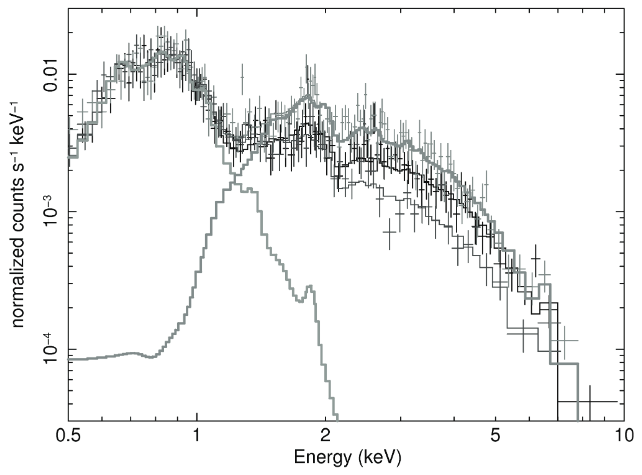
\includegraphics[height=6cm]{figs/tax}
% % % 
\caption{X-ray spectrum of DG~Tau showing the two absorber nature. From \citet{}. \label{fig:tax}}
\end{figure}



\begin{figure}[t]
\centering

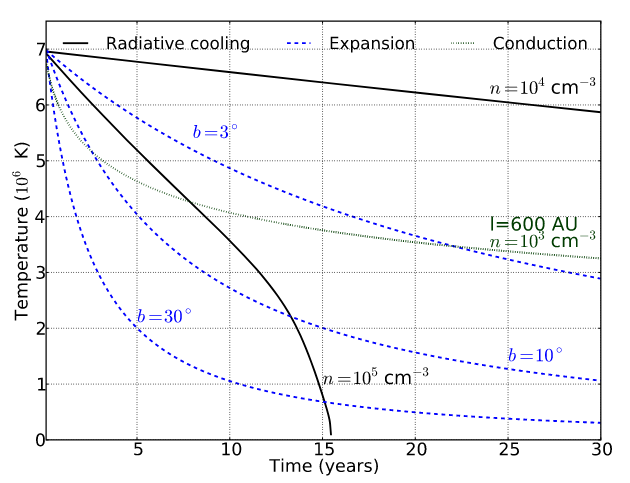
\includegraphics[height=6cm]{figs/cooling}
% % % 
\caption{Cooling of an expanding, X-ray emitting plasma. \label{fig:cooling}}
\end{figure}


{\color{blue}Sabina
Stationary X-ray emission, HH objects

Collimation by the rotating magnetic field or wind pressure

Bonito et al? (HMG: Not a big fan of the setup wit ha ``nozzle'' at the disk which then leads to the diamond shock, but they are often cited and instructuve picture)

Lab work in here, too?
}


\begin{figure}[t]
\centering

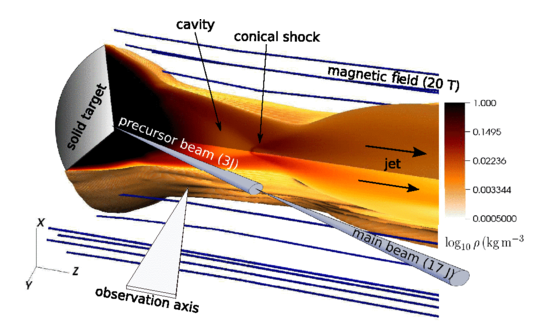
\includegraphics[height=6cm]{figs/lab}
% % % 
\caption{Lab experiment. From \citet{PhysRevLett.119.255002}. \label{fig:lab}}
\end{figure}


\subsection{Connection to other obs}
{\color{blue}Christian

UV obs (DG Tau jet), [Fe II] monitoring, Liu [Ne III]?

Jet rotation

}
